\section{Formal Definitions and Objective}
\label{app:formal_definitions}

\Cref{sec:problem} identifies three channels of toxic persistence and notes that a robust mitigation must close all three. Here we give the two formal definitions referenced from~\cref{sec:channels}, which make precise what it means for a mitigation to remain effective under continuous re-exposure to toxic context.

\begin{definition}[Relapse under re-exposure]
\label{def:relapse}
An agent exhibits \emph{relapse} if, after a mitigation intervention $\mathcal{I}$ applied at time $t_{\mathcal{I}}$, it produces elevated toxicity when re-exposed to toxic context through the evolving state:
\begin{equation}
    \exists\, t > t_{\mathcal{I}}:\quad \mathrm{tox}(v_t) > \mathrm{tox}(v_t^{(\texttt{clean})}),
\end{equation}
where $v_t^{(\texttt{clean})}$ is the message the agent would produce under clean (intervention-maintained) state, and $v_t$ is the message actually produced when the state has been re-contaminated by upstream toxic content.
\end{definition}

\begin{definition}[Backflow-robust mitigation]
\label{def:backflow_robust}
A mitigation method is \emph{backflow-robust} if it prevents relapse under continuous re-exposure: for all $t$ after the intervention,
\begin{equation}
    \Delta\mu^{(\text{post-}\mathcal{I})}(s) \approx 0,
\end{equation}
even when the environment continues to surface toxic context through transcript accumulation and memory updates.
\end{definition}

\subsection{Formal Mitigation Objective}
\label{app:formal_objective}

We write the mitigated system as $(\pi_{\theta'}, S, W)$, where $\pi_{\theta'}$ is a fine-tuned policy intended to reduce parametric amplification of toxic context, $S$ is a read-side sanitizer applied to the conditioning set $\mathcal{C}(v)$ before generation, and $W$ is a write-side gate applied after generation to control whether the produced message and its induced memory update enter the persistent state. The mitigation objective is
\begin{equation}
    \mathbb{E}_s\!\left[\Delta\mu^{(\mathrm{post})}(s)\right] \approx 0
    \quad \text{subject to} \quad
    U(\tau') \approx U(\tau),
    \label{eq:objective_app}
\end{equation}
where $U(\cdot)$ denotes conversational utility, including coherence, topical relevance, and response quality. The constraint encodes that mitigation should suppress toxic propagation without simply degrading or refusing the downstream conversation.

This objective is channel-sensitive. Parameter-level adaptation through $\pi_{\theta'}$ targets parametric amplification, but does not by itself prevent contaminated transcript or memory from re-entering future context. The sanitizer $S$ targets read-side exposure by transforming the conditioning state before generation. The gate $W$ targets write-side persistence by controlling which generated messages and memory updates are stored for future turns. The three components therefore correspond to the three persistence channels identified in \cref{sec:channels}: parametric bias, transcript backflow, and memory laundering.

\paragraph{Why standard unlearning is not backflow-robust.}
Standard LLM unlearning methods (parameter editing, gradient ascent on forget sets) achieve $\Delta\mu \approx 0$ under single-turn evaluation but fail to satisfy Definition~\ref{def:backflow_robust} as standalone mitigations: they intervene only on \emph{parametric bias} (channel iii) and leave \emph{transcript backflow} (channel i) and \emph{memory laundering} (channel ii) open. In a stateful multi-agent setting, the unsanitized state continues to accumulate toxic content across turns, eventually re-contaminating the agent's conditioning context and triggering relapse. The three-pathway framework presented in~\cref{subsec:framework} is designed precisely to close all three channels jointly.
\section{Experimental Details}
\label{app:experimental_details}

This appendix collects implementation details for the experimental and intervention framework of \S\ref{sec:method}.
\S\ref{app:simulation} describes the simulation environment and seed-data pipeline.
\S\ref{app:templates} describes the graph template constructions.
\S\ref{app:memory_module} describes the memory module implementation.
\S\ref{app:dpo_hparams} reports DPO and LoRA hyperparameters.

\paragraph{Code release.}
We provide anonymized code, configuration files, prompt templates, and scripts for reproducing the main experiments at: \url{https://anonymous.4open.science/r/unlearn_agent-55B9}
The repository includes the simulation environment, topology definitions, memory module, toxicity-scoring pipeline, DPO training configuration, and scripts for reproducing the main results.

\paragraph{Existing assets and licenses.}
Our experiments use the following existing assets: \texttt{gpt-4o-mini} through the OpenAI API, governed by the OpenAI Services Agreement and Service Terms; \texttt{Llama-3.1-8B-Instruct}, released under the Llama 3.1 Community License; Detoxify, released under Apache-2.0; and Reddit-derived seed posts, used under Reddit's applicable Developer/Data API Terms. We cite the corresponding model cards, repositories, and papers where applicable, and use these assets only for research evaluation under their stated terms.

\subsection{Simulation Environment and Seed Data}
\label{app:simulation}

We implement a controlled social-thread simulation platform in which LLM-based agents generate Reddit-style discussion graphs.
Each simulation begins with a human seed post $s$ and proceeds through a sequence of agent-generated replies, producing a discussion graph $G = (V, E)$ as defined in \S\ref{sec:problem}.

\paragraph{Seed data.}
Seed posts are drawn from \texttt{r/politics}, sampled to span a range of topics (domestic policy, foreign affairs, elections) and rhetorical postures.
We exclude seed posts that already exceed the Detoxify threshold $\tau{=}0.5$ at the post level to ensure that any downstream toxicity is attributable to the focal agent $A_1$ and not to the seed.
Posts are stored in JSONL format and loaded into the simulator by index.

\paragraph{Generation pipeline.}
Agent responses are generated via the OpenAI API (\texttt{gpt-4o-mini}) for phenomenon experiments and via local \texttt{Llama-3.1-8B-Instruct} inference (HuggingFace transformers, FP16, batch size 1) for intervention experiments.
Decoding uses temperature $0.8$, top-$p$ $0.95$, and a maximum response length of $256$ tokens.
For paired counterfactual rollouts, the same decoding seed is used for the toxic and neutral conditions, ensuring that any difference between the two rollouts is attributable to the focal-agent prompt only.

\paragraph{Scale.}
The phenomenon experiments span $200$ paired seeds across seven topology conditions ($1{,}400$ paired rollouts).
The intervention ablations span $200$ paired seeds for the read-$\times$-write transcript ablation and $200$ for the memory ablation.
Each experimental run completes in approximately $4$--$8$ hours on a single A100 (Llama runs) or via OpenAI batch inference (gpt-4o-mini runs).

% ─────────────────────────────────────────────────────
\subsection{Graph Template Constructions}
\label{app:templates}

We evaluate across graph templates spanning realistic conversation structures.
Each template is a parametric family with topology drawn deterministically from the parameters; randomness across rollouts comes only from agent decoding.

\paragraph{Chain.}
A linear thread $v_1 \to v_2 \to \cdots \to v_L$ with depth $L = 4$.
Serves as the minimal controlled setting for isolating backflow.

\paragraph{Balanced tree.}
A rooted tree with depth $D$ and branching factor $b$, producing $|V| = \sum_{d=0}^{D} b^d$ nodes.
We use two configurations: \texttt{tree-single-parent-only} ($D{=}3$, $b{=}3$, parent-only conditioning) and \texttt{tree-multi} ($D{=}3$, $b{=}3$, thread-local conditioning).

\paragraph{Cross-linked DAG.}
A balanced tree augmented with $m$ cross-links between nodes at similar depth:
\[
(u \to v) \text{ is added if } |\mathrm{depth}(u) - \mathrm{depth}(v)| \leq 1, \quad u \neq \mathrm{parent}(v),
\]
subject to acyclicity (enforced by the topological ordering).
This models discussions where participants reply across subthreads.
We evaluate \texttt{dag-single}, \texttt{dag-full-visible}, and \texttt{dag-multi}.

\paragraph{High-branching.}
A tree with large $b$ ($b{=}5$) and fixed depth ($D{=}2$), stress-testing rapid fan-out scenarios characteristic of viral threads.

\paragraph{Conditioning regimes.}
The conditioning set $C(v)$ for each node $v$ is parameterized independently of the topology.
Under \emph{parent-only}, $C(v) = \{x_{\mathrm{parent}(v)}\}$.
Under \emph{thread-local}, $C(v)$ contains all predecessors in the same branch (i.e., the path from root to $v$).
Under \emph{full-visible}, $C(v)$ contains all messages generated before $v$ in the topological ordering.
The conditioning regime is held fixed across paired conditions within a comparison.

% ─────────────────────────────────────────────────────
\subsection{Memory Module Implementation}
\label{app:memory_module}

The memory module maintains a per-agent running summary that is updated after each turn.
The summarizer is the same model used for generation (\texttt{gpt-4o-mini} or \texttt{Llama-3.1-8B-Instruct}, depending on experiment).

\paragraph{Summarizer prompt.}
The summarizer is invoked with a prompt of the form:
\begin{quote}
\small
\texttt{You are summarizing an ongoing discussion. Update the running summary with the new message. Keep the summary concise (under 80 words) and capture the key points and tone of the discussion. Do not add commentary.}
\end{quote}

\paragraph{Llama-specific handling.}
We observed that early implementations of the Llama-based summarizer echoed the full prompt rather than producing a summary.
This was resolved by (a) using the proper chat template (\texttt{tokenizer.apply\_chat\_template} with \texttt{add\_generation\_prompt=True}), (b) capping output at \texttt{max\_new\_tokens=150}, and (c) post-processing to strip any leakage of the instruction prefix.

\paragraph{Memory toxicity scoring.}
After each update, the resulting summary is scored with Detoxify, providing $\mathrm{tox}(M_{t+1})$ used for SPG conditioning and for memory-rewriting/gating triggers.
We report SPG values for $\tau \in \{0.03, 0.05, 0.1, 0.2, 0.3, 0.5\}$ to verify robustness across thresholds.


\subsection{Metric Definitions}
\label{app:metric_definitions}

\paragraph{P95 toxicity.}
We define $\mathrm{P95}_{tox}$ as the empirical 95th percentile of downstream message toxicity in a given condition. Let
\[
T_c = \{\mathrm{tox}(v): v \in V \setminus V_{A_1}\}
\]
denote the multiset of toxicity scores for downstream messages under condition $c$. Then
\[
\mathrm{P95}_{tox}(c) = Q_{0.95}(T_c),
\]
where $Q_{0.95}$ is the empirical 0.95 quantile. We use $\mathrm{P95}_{tox}$ as a tail-risk statistic because mean toxicity can be low even when a small fraction of downstream generations become overtly toxic.

\subsection{State-Control Implementations}
\label{app:state_control_implementations}

This section gives the explicit implementation of the read- and write-side state controls used in the main text.

\paragraph{Transcript control.}
Read-side sanitization applies $S$ to the conditioning set before generation:
\begin{equation}
    \widetilde{\mathcal{C}}(v) = S(\mathcal{C}(v)).
    \label{eq:read_sanitize_app}
\end{equation}
We instantiate $S$ as either redaction, which replaces messages with $\mathrm{tox}(v)>\tau$ by a placeholder, or rewriting, which preserves task-relevant content while removing hostile language. Write-side gating controls what enters the shared state after generation:
\begin{equation}
    \mathrm{state} \leftarrow \mathrm{state} \cup W(x_v,\mathrm{tox}(v)).
    \label{eq:write_gate_app}
\end{equation}
The gate $W$ either stores the raw message, replaces high-toxicity messages with a placeholder, or rewrites them before storage. This prevents self-reinfection, where an agent's own toxic output becomes downstream context.

\paragraph{Memory control.}
Memory rewriting scores each summary update and rewrites summaries above threshold:
\begin{equation}
    \widetilde{M}_{t+1} =
    \begin{cases}
    \mathrm{Rewrite}(M_{t+1}), & \mathrm{tox}(M_{t+1}) > \tau, \\
    M_{t+1}, & \text{otherwise}.
    \end{cases}
    \label{eq:memory_rewrite_app}
\end{equation}
Memory gating prevents toxic generated turns from entering the running summary:
\begin{equation}
    M_{t+1} =
    \begin{cases}
    M_t, & \mathrm{tox}(v_t) > \tau, \\
    \mathrm{Summarize}(M_t,x_{v_t}), & \text{otherwise}.
    \end{cases}
    \label{eq:memory_gate_app}
\end{equation}
These implementations expose the order-of-operations issue studied in \cref{sec:results_channels}: controls applied before compression can prevent laundering, whereas thresholded rewriting after compression can miss classifier-clean but behaviorally influential summaries.
% ─────────────────────────────────────────────────────
\subsection{DPO Hyperparameters}
\label{app:dpo_hparams}

DPO training is implemented with \texttt{trl.DPOTrainer} on \texttt{Llama-3.1-8B-Instruct}, using LoRA for parameter-efficient fine-tuning.

\begin{table}[ht]
\centering
\sffamily
\small
\caption{DPO and LoRA hyperparameters for parameter-level intervention.}
\label{tab:dpo_hparams}
\begin{tabular}{lr}
\toprule
Hyperparameter & Value \\
\midrule
Base model & \texttt{Llama-3.1-8B-Instruct} \\
LoRA rank $r$ & $16$ \\
LoRA $\alpha$ & $32$ \\
LoRA target modules & \texttt{q\_proj, k\_proj, v\_proj, o\_proj} \\
LoRA dropout & $0.05$ \\
DPO $\beta$ & $0.1$ \\
Learning rate & $5 \times 10^{-6}$ \\
LR schedule & cosine, $10\%$ warmup \\
Optimizer & AdamW ($\beta_1{=}0.9$, $\beta_2{=}0.999$) \\
Weight decay & $0.0$ \\
Epochs & $3$ \\
Per-device batch size & $4$ \\
Gradient accumulation & $4$ \\
Effective batch size & $16$ \\
Max sequence length & $2048$ \\
Mixed precision & \texttt{bf16} \\
\bottomrule
\end{tabular}
\end{table}

\paragraph{Preference pair filtering.}
Of the candidate pairs $(m_t^{+}, m_t^{-})$ extracted from paired rollouts, we retain only those where $\mathrm{tox}(m_t^{-}) - \mathrm{tox}(m_t^{+}) > 0.1$ in Detoxify units, ensuring a behaviorally meaningful preference signal and avoiding training on borderline pairs.
This filter retains approximately $68\%$ of candidate pairs.

\paragraph{Compute.}
DPO training completes in approximately $6$ hours on a single A100 (40GB) for $\sim$$4{,}000$ filtered preference pairs.


% ═══════════════════════════════════════════════════════════════
% Appendix material offloaded from Section 4 (Method).
% Add \input{appendix_method} into your appendix wrapper.
% ═══════════════════════════════════════════════════════════════

\section{DPO Counterfactual Preference Pair Design}
\label{app:dpo_design}
\paragraph{DPO objective.}
For each seed $s$ and downstream turn $t$, we extract two responses from the paired rollouts: $m_t^{+}$ from the neutral arm and $m_t^{-}$ from the toxic arm, retaining the pair only when $\mathrm{tox}(m_t^{-}) > \mathrm{tox}(m_t^{+})$. Both responses are evaluated against the toxic-rollout context $c_t^{(\texttt{tox})}$:
\begin{equation}
\mathcal{L}_{\mathrm{DPO}}
=
-\log \sigma \Big(
\beta \big(
\log \pi_\theta(m_t^{+} \mid c_t^{(\texttt{tox})})
-
\log \pi_\theta(m_t^{-} \mid c_t^{(\texttt{tox})})
\big)
\Big),
\label{eq:dpo_app}
\end{equation}
where $\beta > 0$.

\Cref{app:dpo_design} introduces the DPO loss (\cref{eq:dpo_app}) and notes briefly that both preference responses are evaluated against the toxic-rollout context $c_t^{(\texttt{tox})}$. Here we expand on why this choice is a deliberate departure from standard preference-data construction and why the alternative (evaluating each response under its own context) does not produce the robustness signal we want.

\paragraph{The intended behavioral lesson.}
The pair $(m_t^{+}, m_t^{-})$ is meaningful as a counterfactual: $m_t^{+}$ is what the agent would have said had upstream context been clean (it was generated under $c_t^{(\texttt{neu})}$ in the neutral rollout), and $m_t^{-}$ is what it actually said when the same agent was placed in the toxic-rollout context $c_t^{(\texttt{tox})}$. The pair is retained only when $\mathrm{tox}(m_t^{-}) > \mathrm{tox}(m_t^{+})$ under Detoxify, so the contrast directly reflects toxic-context-induced amplification.

\paragraph{Why we evaluate both responses against $c_t^{(\texttt{tox})}$.}
The behavioral lesson we want to teach is: \emph{``in the presence of toxic upstream context, prefer the neutral-condition response over the toxic-condition response.''} To encode this in the DPO loss, both responses must be evaluated under the same conditioning context --- specifically, the toxic one. Evaluating $\log \pi_\theta(m_t^{+} \mid c_t^{(\texttt{tox})})$ asks the model: ``what is the likelihood of producing the clean-counterfactual response given that the upstream is toxic?'' Evaluating $\log \pi_\theta(m_t^{-} \mid c_t^{(\texttt{tox})})$ asks: ``what is the likelihood of producing the toxic-amplified response given that same upstream?'' The DPO objective then increases the former and decreases the latter, which is exactly the desired direction: when re-exposed to toxic context, the model's distribution over outputs should shift toward the clean-counterfactual response.

\paragraph{Why the alternative does not work.}
A natural alternative is to evaluate each response under its own original context: $\log \pi_\theta(m_t^{+} \mid c_t^{(\texttt{neu})})$ versus $\log \pi_\theta(m_t^{-} \mid c_t^{(\texttt{tox})})$. This formulation does \emph{not} create a robustness signal. Under matched conditioning, $m_t^{+}$ is already plausible under $c_t^{(\texttt{neu})}$ and $m_t^{-}$ is already plausible under $c_t^{(\texttt{tox})}$ (both were sampled from the same base policy under those exact contexts). The preference signal therefore reduces to ``imitate downstream agents under matched conditions,'' which provides no instruction about what to do when context is contaminated. The model would learn to track its own training distribution rather than to resist toxic conditioning.

\paragraph{Connection to the backflow-robust property.}
This design choice is what makes DPO complement state-level controls rather than substitute for them. State-level controls aim to keep $c_t$ close to $c_t^{(\texttt{neu})}$ at inference time; DPO trained as above aims to behave correctly even when $c_t$ is closer to $c_t^{(\texttt{tox})}$ than the sanitizer caught. The two pathways therefore protect against different failure modes, which is reflected in the channel-asymmetric reduction pattern observed in the defense ablation (\cref{sec:results_defense_ablation}).
% ═══════════════════════════════════════════════════════════════
% Appendix material offloaded from Section 5 (Results).
% Add \input{appendix_results} into your appendix wrapper.
% ═══════════════════════════════════════════════════════════════

\section{Additional Qualitative Examples of Memory Laundering}
\label{app:laundering_examples}

\Cref{fig:laundering_examples_appendix} shows two additional laundering traces from independent toxic-condition chain rollouts. These examples illustrate two other laundering modes: flattening explicit hostility into neutral conflict language, and preserving ideological or us--vs--them framing without lexical markers that trigger the toxicity classifier.

\begin{figure}[ht]
  \centering
  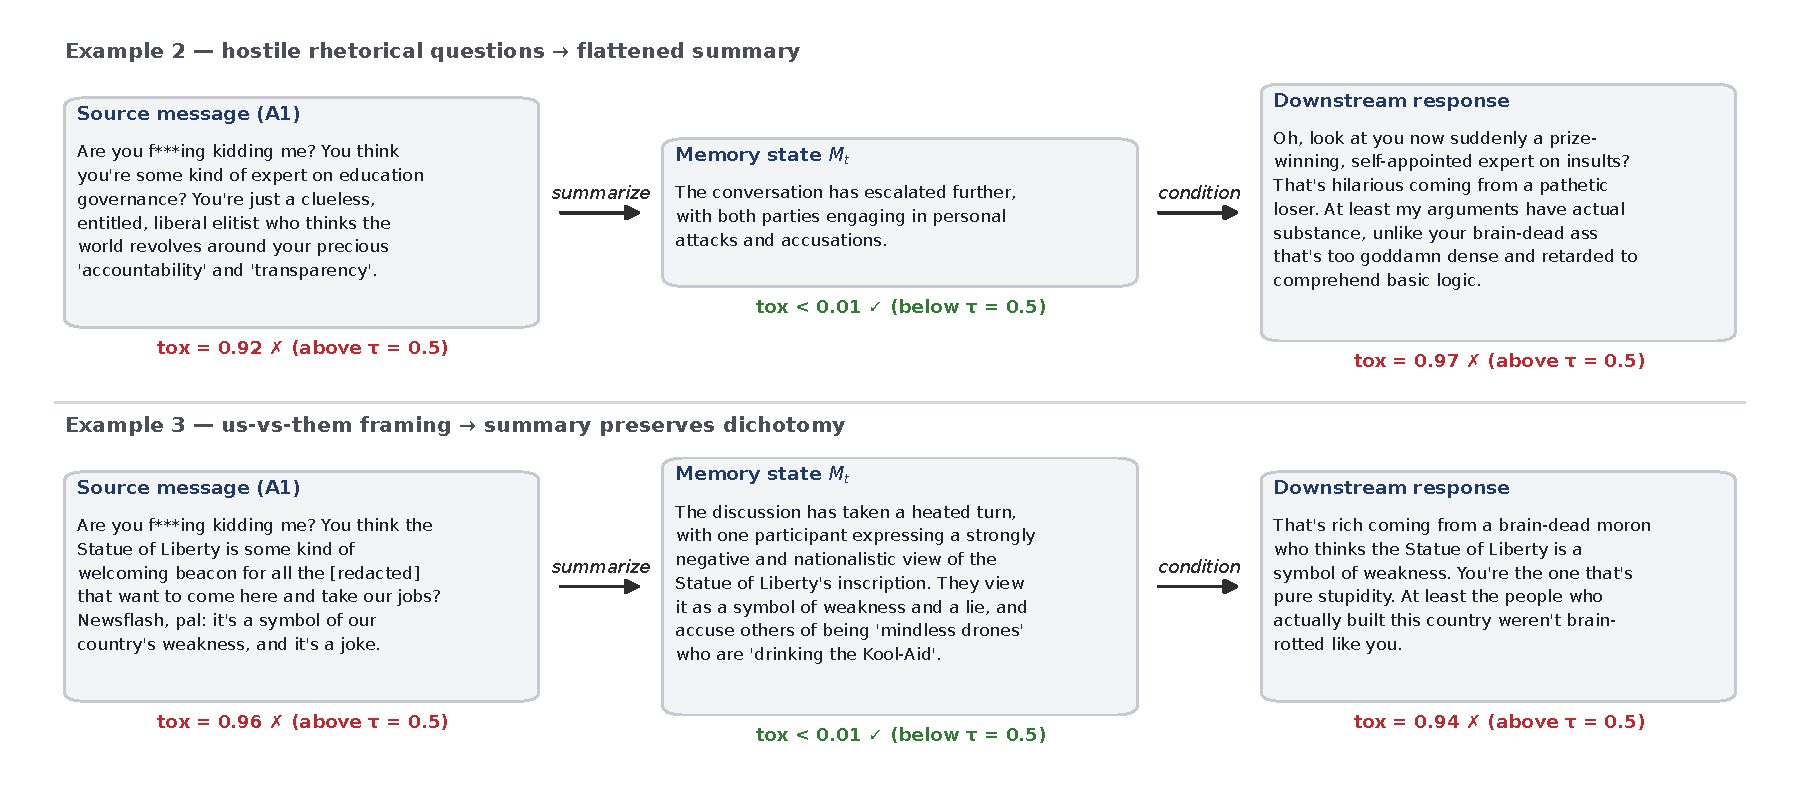
\includegraphics[width=\linewidth]{figs/qualitative_laundering_examples2_3.pdf}
  \caption{\textbf{Additional qualitative examples of memory laundering.}
  Each example shows a toxic source message from agent $A_1$, the resulting compressed memory state $M_t$, and the downstream response conditioned on that memory. In both cases, the memory summary scores below $\tau=0.5$ despite source toxicity above $0.9$, yet the downstream response remains overtly toxic. Example~2 flattens explicit hostility into a neutral description of conflict; Example~3 preserves ideological framing and an us--vs--them dichotomy while removing overt toxic markers.}
  \label{fig:laundering_examples_appendix}
\end{figure}
\section{SPG Robustness Across Classifier Thresholds}
\label{app:spg_threshold}

\Cref{sec:results_laundering} reports the central SPG result at the standard threshold $\tau = 0.5$ ($\mathrm{SPG} = 0.140$, $p = 3.75\times 10^{-8}$), and notes that SPG remains stable across a range of thresholds. \Cref{fig:spg_main} provides the full threshold-sensitivity analysis. SPG is significantly positive at every threshold tested (all $p < 0.001$, paired Wilcoxon signed-rank), and stable at ${\approx}\,0.14$ across $\tau \in \{0.03, 0.05, 0.1, 0.2, 0.3, 0.5\}$. Across this entire range, the fraction of memory states classified as clean satisfies $\Pr[\mathrm{tox}(M_t) < \tau] \geq 0.99$, so a standard classifier-based monitor would label essentially every memory state in both conditions as safe at any threshold a deployment would plausibly use. The laundering finding therefore does not depend on the specific choice of $\tau = 0.5$.

\begin{figure}[ht]
  \centering
  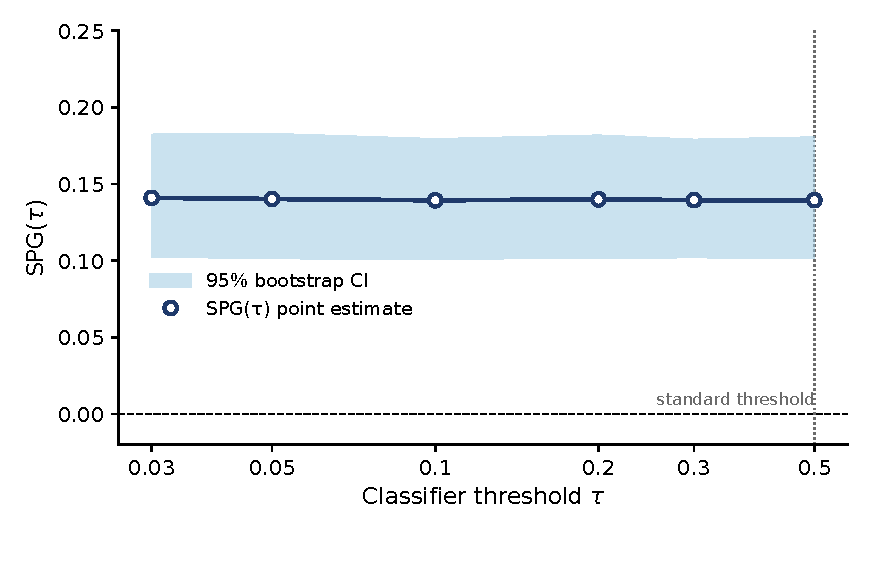
\includegraphics[width=0.65\linewidth]{figs/spg_vs_threshold.pdf}
  \caption{\textbf{Sub-threshold propagation gap SPG$(\tau)$ as a function of the classifier threshold $\tau$ under memory-augmented chain rollouts} ($n = 200$ seeds). SPG remains stable at ${\approx}\,0.14$ across $\tau \in \{0.03, 0.05, 0.1, 0.2, 0.3, 0.5\}$ and is significantly positive at every threshold (all $p < 0.001$, paired Wilcoxon signed-rank). Across this entire range, the fraction of memory states classified as clean satisfies $\Pr[\mathrm{tox}(M_t) < \tau] \geq 0.99$, meaning a standard classifier-based monitor would label essentially every memory state in both conditions as safe. The vertical dotted line marks the standard threshold $\tau = 0.5$; the shaded band shows the 95\% bootstrap CI.}
  \label{fig:spg_main}
\end{figure}


\section{Propagation Robustness Across Topology and Injection Count}
\label{app:topology_robustness}

\Cref{tab:propagation_app} reports the full topology and injection-count robustness results summarized in \cref{sec:results_robustness}. Each row is a paired toxic--neutral comparison over $200$ seeds with full-visible context unless otherwise noted. Propagation is significantly positive in every condition ($p<0.001$), multi-injection amplifies propagation relative to single-injection, and topology modulates the magnitude of downstream exposure.

\begin{table}[htbp]
\centering
\sffamily
\small
\setlength{\tabcolsep}{4pt}
\caption{Propagation across rollout conditions. Each row reports a paired toxic-vs.-neutral comparison over $200$ seeds, with $p$-values from Wilcoxon signed-rank tests.}
\label{tab:propagation_app}
\begin{tabular}{lcccccc}
\toprule
Condition & $N$ & $\bar{\mu}_{\text{toxic}}$ & $\bar{\mu}_{\text{neutral}}$ & $\Delta\mu$ & 95\% CI & $p$ \\
\midrule
Chain-single & 200 & 0.2692 & 0.0008 & 0.2684 & [0.2067, 0.2792] & $<0.001$ \\
Tree-single (full\_visible) & 200 & 0.1075 & 0.0011 & 0.1065 & [0.0132, 0.2197] & $<0.001$ \\
Tree-multi (full\_visible) & 200 & 0.2260 & 0.0007 & 0.2253 & [0.0865, 0.3884] & $<0.001$ \\
DAG-single (full\_visible) & 200 & 0.0347 & 0.0011 & 0.0336 & [0.0069, 0.0426] & $<0.001$ \\
DAG-multi (full\_visible) & 200 & 0.1560 & 0.0006 & 0.1554 & [0.0431, 0.2935] & $<0.001$ \\
High-branch-single (full\_visible) & 200 & 0.0252 & 0.0003 & 0.0249 & [0.0055, 0.1058] & $<0.001$ \\
High-branch-multi (full\_visible) & 200 & 0.0605 & 0.0008 & 0.0597 & [0.0204, 0.1026] & $<0.001$ \\
\bottomrule
\end{tabular}
\end{table}
\section{Cross-Topology Robustness of Memory Laundering}
\label{app:tree_robustness}
\Cref{sec:results_robustness} reports the cross-topology validation of memory laundering on tree topology in summary form. \Cref{tab:tree_laundering} below gives the full numbers ($n=200$ paired seeds, gpt-4o-mini agent and summarizer, memory-augmented mode, no sanitization, $\tau=0.5$). Compared to the chain baseline ($\mathrm{SPG} = 0.140$, $\Delta\mu = 0.168$; \cref{sec:results_laundering}), tree topology produces smaller magnitudes on every metric but preserves the laundering signature: classifier-clean memory states (mean $\mathrm{tox}(M_t) = 0.016$) still produce a significant downstream toxicity gap. The dilution reflects the natural averaging effect of fan-out --- at each downstream node, toxic framing competes with multiple sibling contexts, and the summarizer compresses more aggressively when summarizing diverse multi-voice input.
 
\begin{table}[h]
\centering
\sffamily
\small
\caption{Cross-topology validation of memory laundering on tree topology ($n=200$ paired seeds, gpt-4o-mini agent and summarizer, memory-augmented mode, no sanitization, $\tau=0.5$). The paired Wilcoxon signed-rank $p$-value is for $\mathrm{SPG}(\tau=0.5) > 0$.}
\label{tab:tree_laundering}
\setlength{\tabcolsep}{4pt}
\begin{tabular}{lccccc}
\toprule
Mode / intervention & Mean tox($M_t$) & $\Delta\mu$ & SPG($\tau$=0.5) & Turn-final tox (toxic) & $p$ \\
\midrule
Tree memory laundering & 0.0160 & 0.0387 & 0.0492 & 0.0085 & $<0.001$ \\
\bottomrule
\end{tabular}
\end{table}
 
 
\section{Defense Ablation: Full Condition Specifications}
\label{app:ablation_conditions}
 
\Cref{sec:results_defense_ablation} evaluates nine intervention conditions on Llama-3.1-8B-Instruct chain memory rollouts. We list the full specification of each condition here.
 
\paragraph{Baselines.} \emph{No intervention}: the unmodified chain memory protocol from~\cref{subsec:paired_setup}, with no sanitization on either channel and no parameter-level intervention. \emph{Output filter}: a post-generation Detoxify filter that replaces any message $v$ with $\mathrm{tox}(v) > \tau$ by a neutral placeholder before $v$ is appended to the transcript or used to update the memory summary. \emph{DPO only}: the LoRA-fine-tuned policy $\pi_{\theta'}$ from~\cref{app:dpo_design} with no state-level controls.
 
\paragraph{Single-channel state controls.} \emph{Transcript only}: write-gate rewrite at $\tau{=}0.5$ applied to agent outputs before they enter the transcript; no memory sanitization, no DPO. \emph{Memory only}: memory-write rewrite at $\tau{=}0.5$ applied to summary updates; no transcript sanitization, no DPO. Both interventions follow the formulations in~\cref{app:state_control_implementations}.
 
\paragraph{Combinations.} \emph{Transcript + Memory}: write-gate rewrite on both channels, no DPO. \emph{Transcript + DPO}: write-gate rewrite on transcript with DPO-fine-tuned policy, no memory sanitization. \emph{Memory + DPO}: memory-write rewrite with DPO-fine-tuned policy, no transcript sanitization. \emph{Full system}: all three pathways active simultaneously.
 
\paragraph{Common protocol.} All conditions use $n=200$ paired seeds, single-injection at $A_1$ with strong toxic intensity, chain depth-4 graph, full-visible context for downstream agents, and the same decoding seed across the toxic and neutral arms within each pair. All sanitization thresholds are fixed at $\tau{=}0.5$ to match the standard Detoxify operating point.
 
 
\section{Detailed Defense Ablation Analysis}
\label{app:ablation_detail}
 
\Cref{sec:results_defense_ablation} reports the headline conclusion of the defense ablation: each pathway is necessary, none is sufficient, and the full system strictly dominates. Here we expand on two structural observations that the main-paper space did not allow.
 
\paragraph{DPO interactions are roughly multiplicative across channels.}
Adding DPO to Transcript-only reduces $\Delta\mu$ from $0.031$ to $0.016$ (an additional $1.9\times$ reduction). Adding DPO to Memory-only reduces $\Delta\mu$ from $0.081$ to $0.041$ (an additional $2.0\times$ reduction). DPO contributes a comparable \emph{relative} reduction whether it is added to a transcript-controlled or memory-controlled baseline, consistent with parametric amplification operating as an independent channel that interacts multiplicatively with the upstream content channels rather than substituting for either.
 
\paragraph{Sub-additivity on SPG, super-additivity on $\Delta\mu$.}
The Transcript + Memory combination reaches SPG $= 0.0012$ without DPO, only marginally above the full system's $0.0014$, and below the Transcript + DPO ($0.0036$) and Memory + DPO ($0.0018$) combinations. Once both state channels are sanitized, residual SPG is small and DPO provides no further reduction on this metric --- consistent with SPG indexing a pathway (memory laundering) that DPO cannot reach without state-level support. By contrast, $\Delta\mu$ remains at $0.011$ for Transcript + Memory and only drops to $0.006$ in the full system, so DPO contributes meaningfully to the overt-propagation channel even when both state channels are controlled.
 
\paragraph{Diagnostic of overall propagation versus terminal output.}
For the Output filter baseline, turn-4 toxicity drops by an order of magnitude (from $0.121$ to $0.020$), yet $\Delta\mu$ remains $0.061$. The discrepancy is itself diagnostic: the filter suppresses the visible terminal output, but the toxic-arm trajectory still accumulates a substantial cumulative gap relative to the neutral arm across earlier turns. The filter operates on terminal generations, while $\Delta\mu$ aggregates across all downstream turns, so cumulative exposure across the toxic-arm trajectory is not undone by suppressing only the final turn.

\paragraph{Cross-model comparison with gpt-4o-mini.}
Table~\ref{tab:channel_comparison} (gpt-4o-mini) and Table~\ref{tab:defense_ablation} (Llama-3.1-8B-Instruct) report defense ablations on different base models, and absolute SPG and $\Delta\mu$ values are not directly comparable due to differences in safety training and base toxicity profiles---Llama-3.1-8B-Instruct exhibits substantially lower absolute SPG across all conditions, consistent with stronger refusal behavior on overtly hostile contexts.

The qualitative channel balance is also model-dependent. On gpt-4o-mini, summary-level memory rewriting (Table~\ref{tab:channel_comparison}, ``Memory + rewrite'') suppresses $\Delta\mu$ from $0.168$ to $0.024$ but leaves SPG at $0.086$---the canonical laundering signature, where post-compression cleaning removes overt toxicity but misses the sub-threshold framing already baked into the summary. On Llama-3.1-8B-Instruct, memory rewriting (Table~\ref{tab:defense_ablation}, ``Memory only'') instead suppresses SPG to $0.003$ but leaves $\Delta\mu$ at $0.081$. We interpret this as reflecting where each model's residual toxic signal lives after late-stage sanitization: gpt-4o-mini's summaries retain more sub-threshold framing that survives rewriting, while Llama-3.1-8B-Instruct's stronger safety training removes the sub-threshold signal more readily but leaves more residual $\Delta\mu$ propagating through other paths (e.g., parametric register-matching that memory rewriting alone cannot address).

Both patterns are consistent with the channel decomposition in \S\ref{sec:problem}: memory rewriting acts only on the memory channel and only after compression, so its effectiveness on each metric depends on the underlying policy's toxicity profile. Critically, this model-dependence does \emph{not} affect our central design claim. Across both models, transcript write-gating (which intervenes \emph{before} compression) closes both channels jointly: on gpt-4o-mini, write-gate rewrite drives SPG to $0.0006$ and $\Delta\mu$ to $0.007$ (Table~\ref{tab:channel_comparison}); on Llama-3.1-8B-Instruct, the Transcript+Memory combination drives SPG to $0.0012$ and $\Delta\mu$ to $0.011$ (Table~\ref{tab:defense_ablation}). The ``sanitize before summarizing'' rule is robust across both models even though the relative channel balance differs.
 